%%%%%%%%%%%%%%%%%%%%%%%%%%%%%%%%%%%%%%%%%%%%%%%%%%%%%%%%%%%%%%%%%%%%%%%%%%%%%%%%
%2345678901234567890123456789012345678901234567890123456789012345678901234567890
%        1         2         3         4         5         6         7         8

%\documentclass[letterpaper, 10 pt, conference]{ieeeconf}  % Comment this line out if you need a4paper

\documentclass[a4paper, 10pt, conference]{ieeeconf}      % Use this line for a4 paper

%\IEEEoverridecommandlockouts                              % This command is only needed if 
                                                          % you want to use the \thanks command

\overrideIEEEmargins                                      % Needed to meet printer requirements.

% The following packages can be found on http:\\www.ctan.org
\usepackage{subfigure}
\usepackage[OT1]{fontenc} 
\usepackage{graphicx} % for pdf, bitmapped graphics files
\usepackage{multirow}
%\usepackage{epsfig} % for postscript graphics files
%\usepackage{mathptmx} % assumes new font selection scheme installed
%\usepackage{times} % assumes new font selection scheme installed
%\usepackage{amsmath} % assumes amsmath package installed
%\usepackage{amssymb}  % assumes amsmath package installed

\title{\LARGE \bf
Off-Road Drivable Area Extraction Using 3D LiDAR Data
}


\author{\authorblockN
	{Biao Gao\authorrefmark{1},
		Anran Xu\authorrefmark{1}, 
		Yancheng Pan\authorrefmark{1},
		Xijun Zhao\authorrefmark{2},
		Wen Yao\authorrefmark{2},
		Huijing Zhao\authorrefmark{1}}
	\authorblockA{\authorrefmark{1}Peking University, Beijing, China}
	\authorblockA{\authorrefmark{2}China North Vehicle Research Institute, Beijing, China}}

\begin{document}


\maketitle


%%%%%%%%%%%%%%%%%%%%%%%%%%%%%%%%%%%%%%%%%%%%%%%%%%%%%%%%%%%%%%%%%%%%%%%%%%%%%%%%
\begin{abstract}
	
nothing.

\end{abstract}


%%%%%%%%%%%%%%%%%%%%%%%%%%%%%%%%%%%%%%%%%%%%%%%%%%%%%%%%%%%%%%%%%%%%%%%%%%%%%%%%
\section{INTRODUCTION}

nothing.

\section{RELATED WORKS}

nothing.

\begin{figure}[ht]
	\centering
	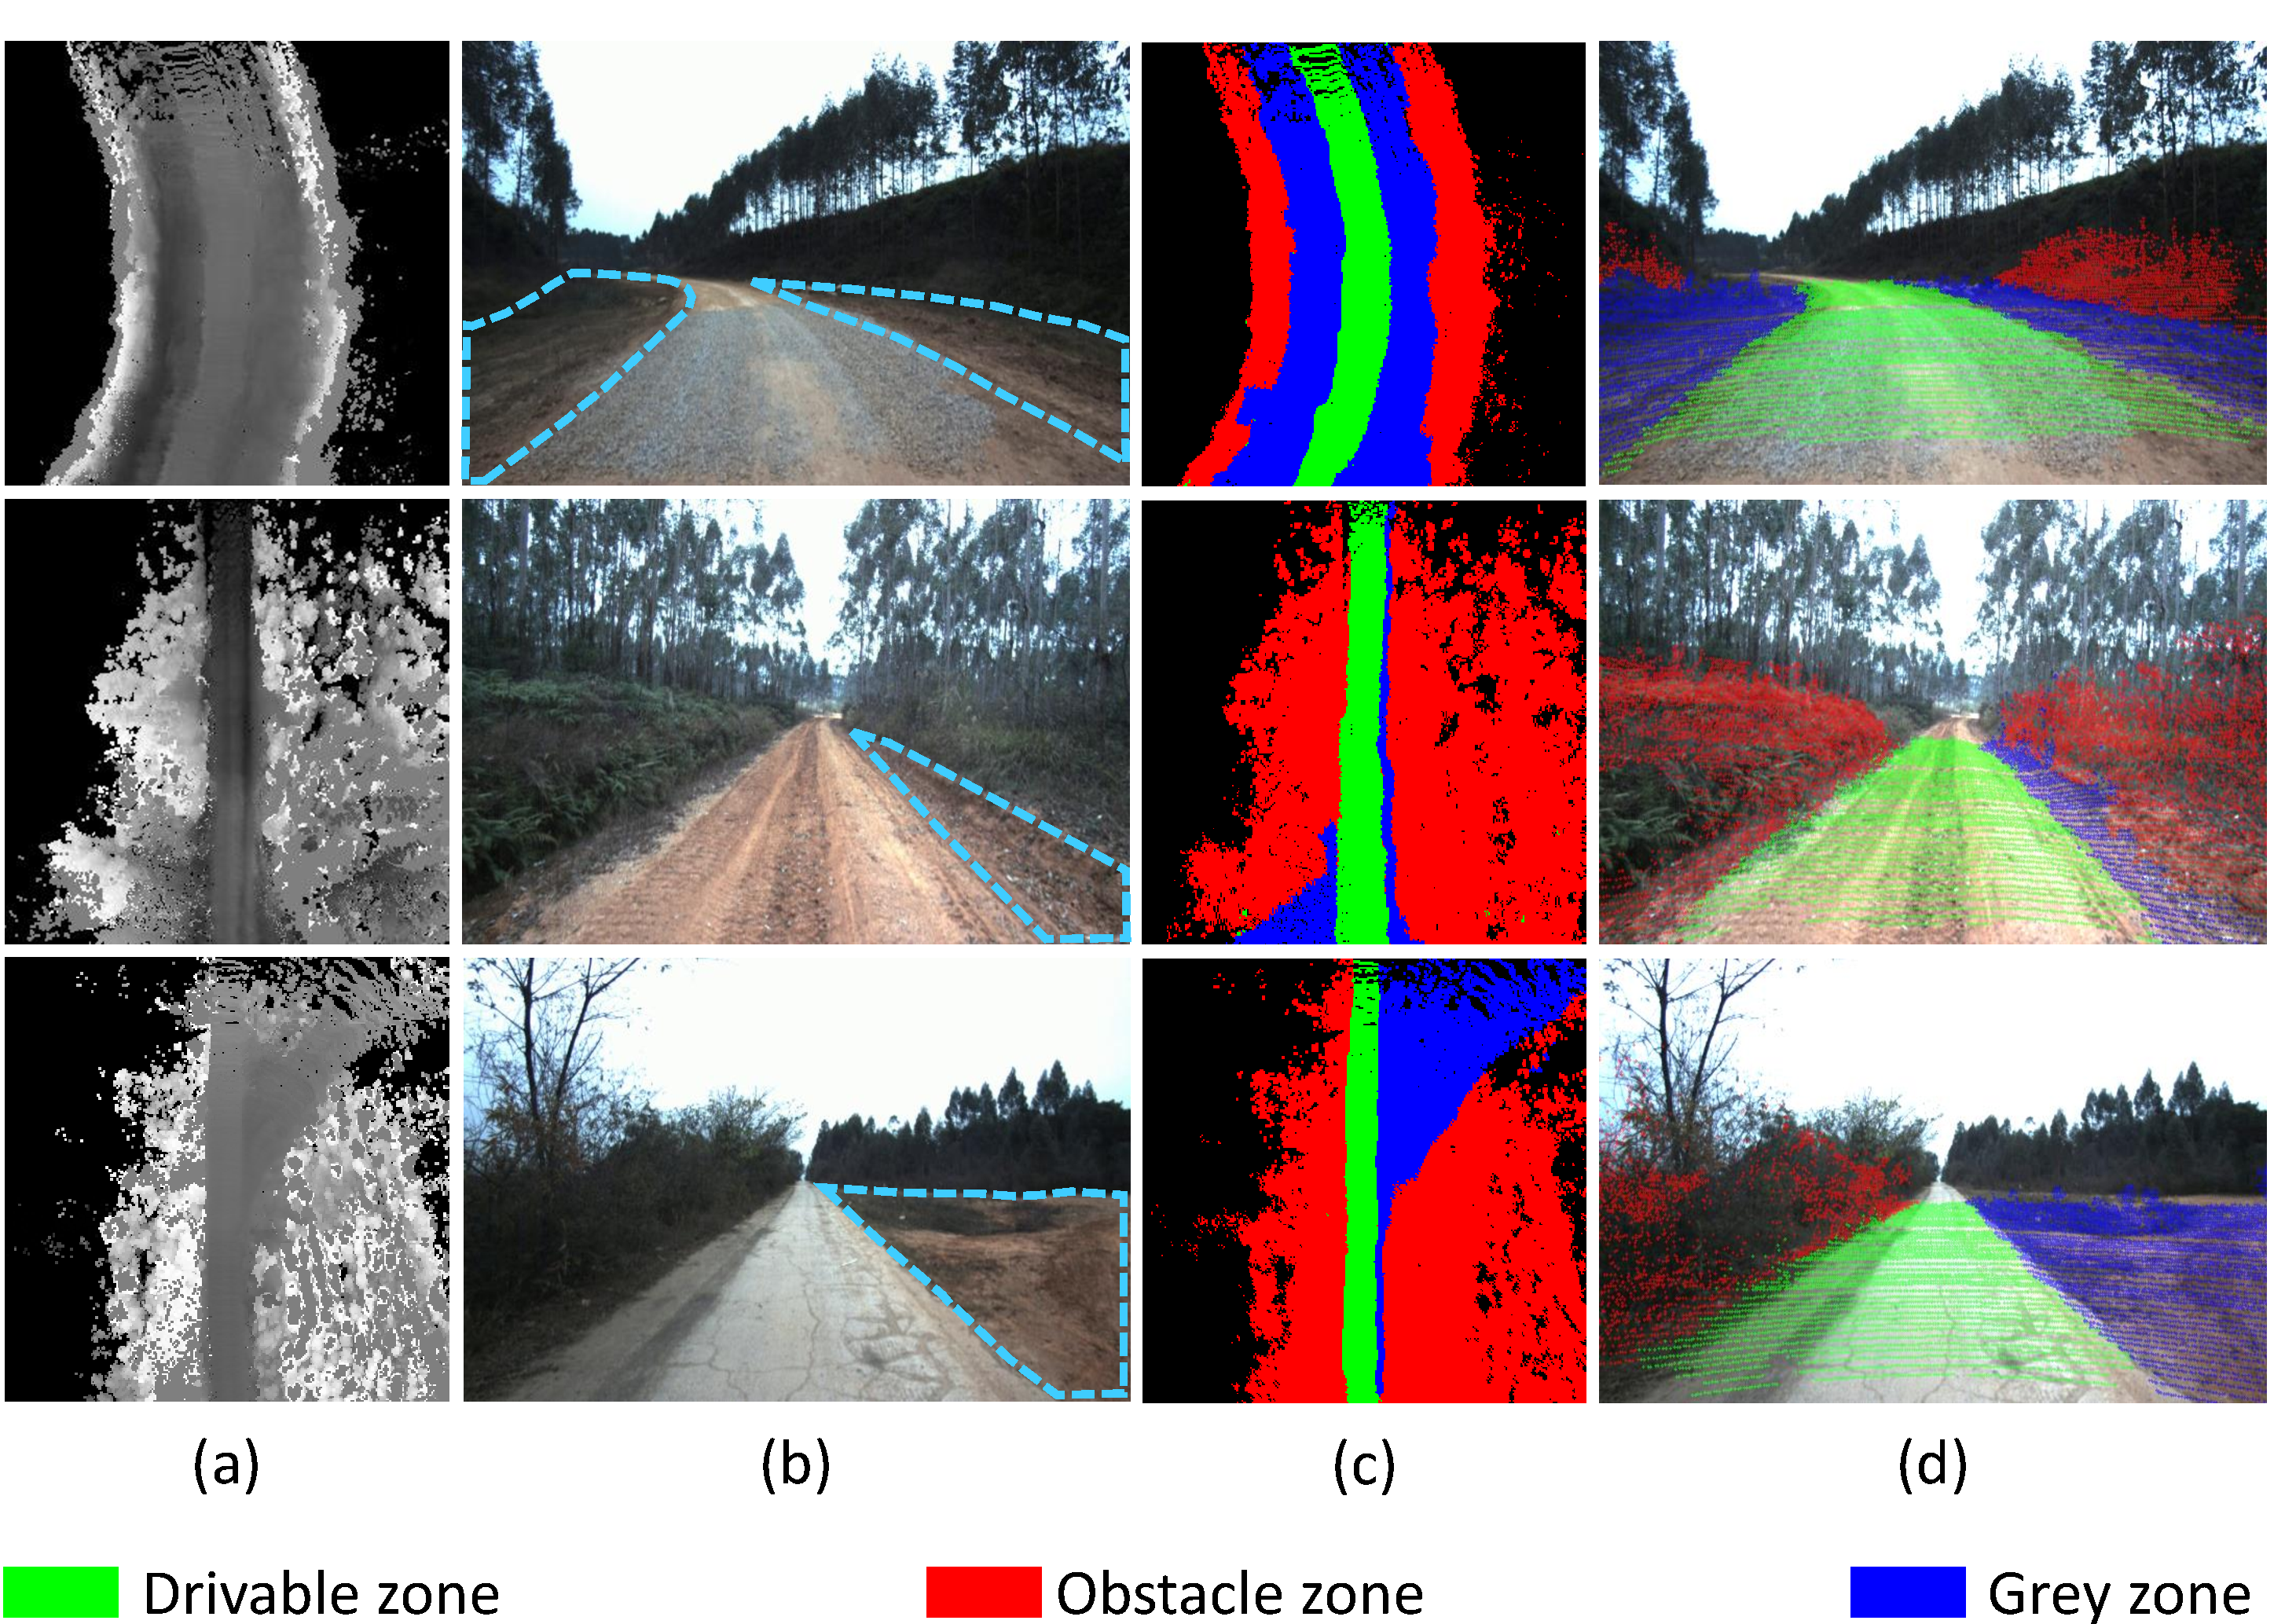
\includegraphics[scale=0.175]{offRoadExample.pdf}
	\caption{The ambiguities in off-road drivable area extraction. (a) Input LiDAR data in bird's-eye view. (b) Image reference of input data. (c) Human annotation. (d) Projected point clouds in camera coordinate.}
	\label{fig:example}
\end{figure}

\section{METHODOLOGY}

\subsection{Problem Definition}

Let's denote the origin point clouds from 3D LiDAR sensor as $PC={\{pt_i\}}_{0\le i<N}$, where $N$ is the number of points. We aggregate a few frames' point clouds to get a dense bird's-eye view height map $X=\{x_{j,k}\}_{0\le j<H,0\le k<W}$, which is used as our input data format. The input height map is in the size of $H\times W$ and each pixel $x_{j,k}$ means the physical height of pixel $(j,k)$. The examples of input can be seen in Fig.\ref{fig:example}(a).

Different from the well-defined road borders in structured urban environment, the main peculiarity in off-road environment is the ambiguous area beside the road margin, which is called grey zone. In order to distinguish it with others, we let $Label Set=\{unknown,drivable\ zone,obstacle\ zone,grey\ zone\}$, and we use $G=\{g_{j,k}\}_{0\le j<H,0\le k<W}$ to denote human annotated ground truth, where $g_{j,k}\in LabelSet$.

The origin output of our proposed framework is a cost map $C=\{c_{j,k}\}_{0\le j<H,0\le k<W}$, where each $c_{j,k}\in [0,1]$ evaluates the traversability cost of pixel $(j,k)$. Our proposed framework learns a mapping from input $X$ to cost map $C$.

\begin{equation}
f_\theta^*:x_{j,k}\rightarrow c_{j,k} \in [0,1]
\end{equation}

For the convenience of comparison with human-annotated ground truth $G$ and other baseline methods, we use $d_\alpha$ to remap cost map $C$ to label $Y=y_{j,k}\in LabelSet$.

\begin{equation}
d_\alpha:c_{j,k}\rightarrow y_{j,k} \in LabelSet
\end{equation}

Therefore, the problem of this work can be formulated as learning a multi-class classifier $f_\theta=d_\alpha(f_\theta^*)$ that maps input $x_{j,k}$ to a label $y_{j,k}\in LabelSet$.

\subsection{Network Architecture}

Due to the ambiguity of the grey zone, we hold the view that classifying it as an independent label from the others is not reasonable enough. In some cases, the grey zone is drivable technically but not human-desired, which is very close or even overlapped with the drivable zone in feature space. In other cases, the grey zone may have higher traversability cost than common drivable zone, which is closer or even overlapped with the obstacle zone in feature space. As a result, viewing the ambiguous grey zone as an independent label in training process will cause confusion for the deep learning model, and the experimental results in Sec.\ref{sec:experiment} give the evidence of this viewpoint.

Therefore, we can assume that the samples of grey zone are distribute between the drivable samples and the obstacle samples in feature space. The key idea of our proposed method is learning two classification surfaces in feature space and use the margin between them to split the grey zone samples. One classification surface is used to separate the drivable zone samples from others. The other one is used to separate the obstacle zone samples. We can evaluate the traversability cost of a sample by its feature distance to the two surfaces.

\begin{figure}[!h]
	\centering
	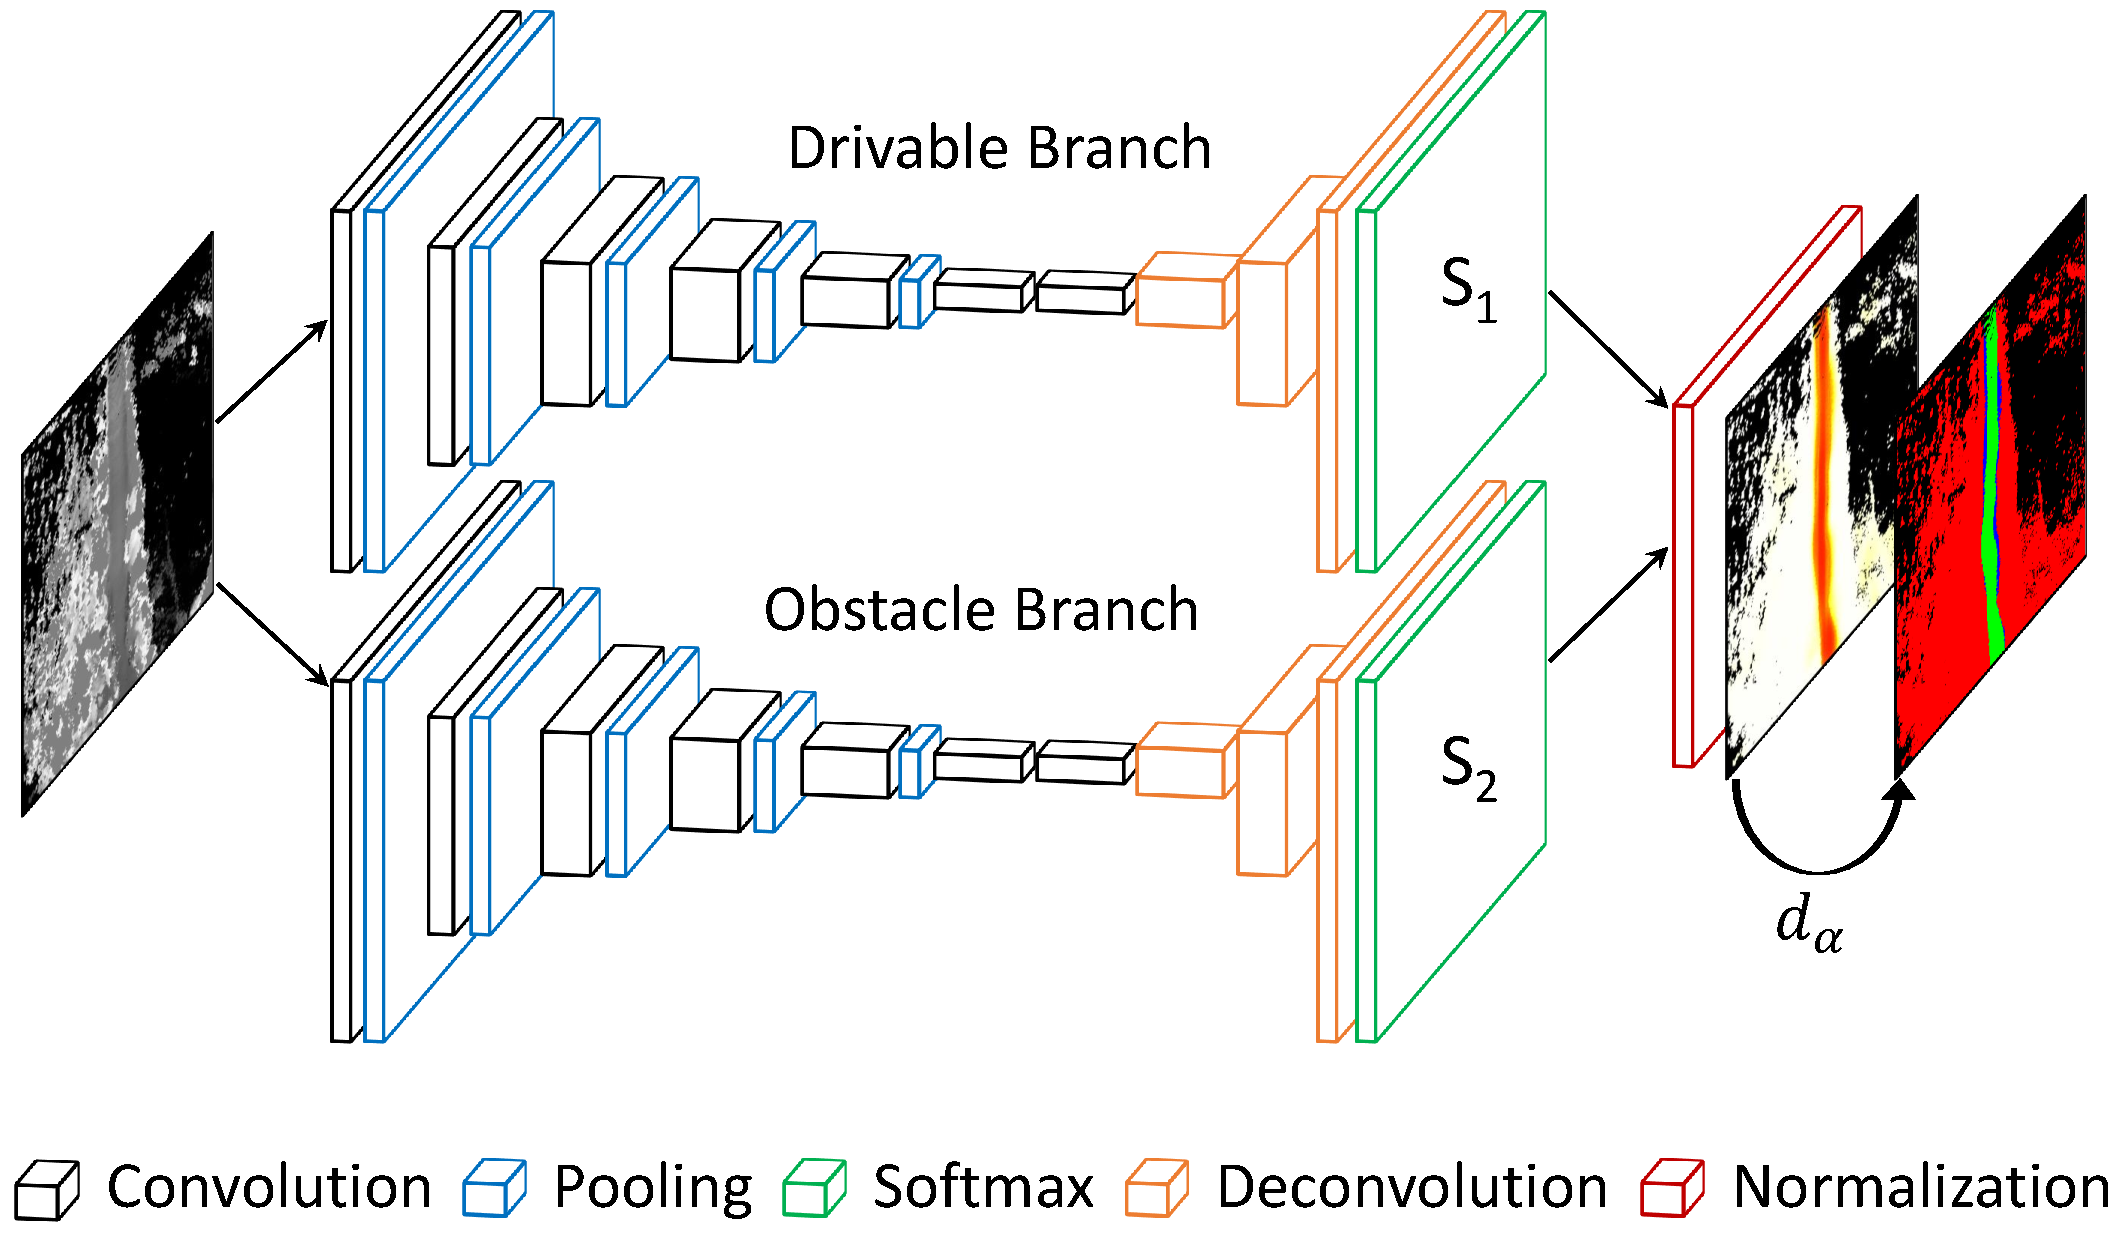
\includegraphics[scale=0.23]{network.pdf}
	\caption{Network}
	\label{fig:network}
\end{figure}

As shown in Fig.\ref{fig:network}, the proposed network has two branches in order to learn the two classification surfaces mentioned above. Both of them are designed according to the common VGG-based fully convolutional network. The difference is that the last layer does not output the discrete labels but the probabilistic predictions from the last softmax layer. We denote them as $S_1$ and $S_2$, which are in the range of $[0,1]$.

Each branch is trained end-to-end guided by the following cross entropy loss function:
\begin{equation}
\label{equ:loss0}
L^{br}(X;\Theta^{br})=-\sum_{i}{y_i^{br} \log{P(y_i^{br}|\Theta^{br})}}, \ br \in \{dri, obs\}
\end{equation}
where $br\in\{dri, obs\}$ is the name of network's branch. $P(y_i^{br}|\Theta^{br})$ is the probability that  pixel $i$ is predicted as label $y_i^{br}$ with the network parameters $\Theta^{br}$. We use $dri,obs$ and $gre$ to represent $drivable, obstacle$ and $grey\ zone$.

When training the network, different label $y_i^{br}$ is used in the two branches. 
\begin{equation}
y_i^{br}= 
\left\{
\begin{array}{ll}
\Psi(\vec{br}), &\quad if \ g_i = gre \\ 
\vec{g_i} &\quad if \ g_i \in \{dri,obs \} \\
\end{array}
\right.
\end{equation}
where $\vec{br}$ is the one-hot vector of label $br\in\{dri, obs\}$. $\Psi(\vec{dri})=\vec{obs}$ and $\Psi(\vec{obs})=\vec{dri}$. For example, we replace all the pixels with ground truth $g_i=gre$ to the label $obs$ to get $y_i^{dri}$ when training the drivable branch.

We use the following regulation to calculate the traversability cost map $C$ and then get the discrete label:

\begin{equation}
C= 
\left\{
\begin{array}{ccc}
S_1, &\  if \ S_1>\alpha_1 \\ 
1-S_2, &\ if \ S_2>\alpha_2 \\
\frac{1-S_2}{1-S_1 + 1-S_2}, &\ otherwise
\end{array}
\right.
\end{equation}

where the pixels satisfied the first condition will be labeled as $drivable\ zone$, the second is $obstacle\ zone$ and the last is $grey\ zone$.

\subsection{Semi-supervised Learning}

\begin{figure*}[ht]
	\centering
	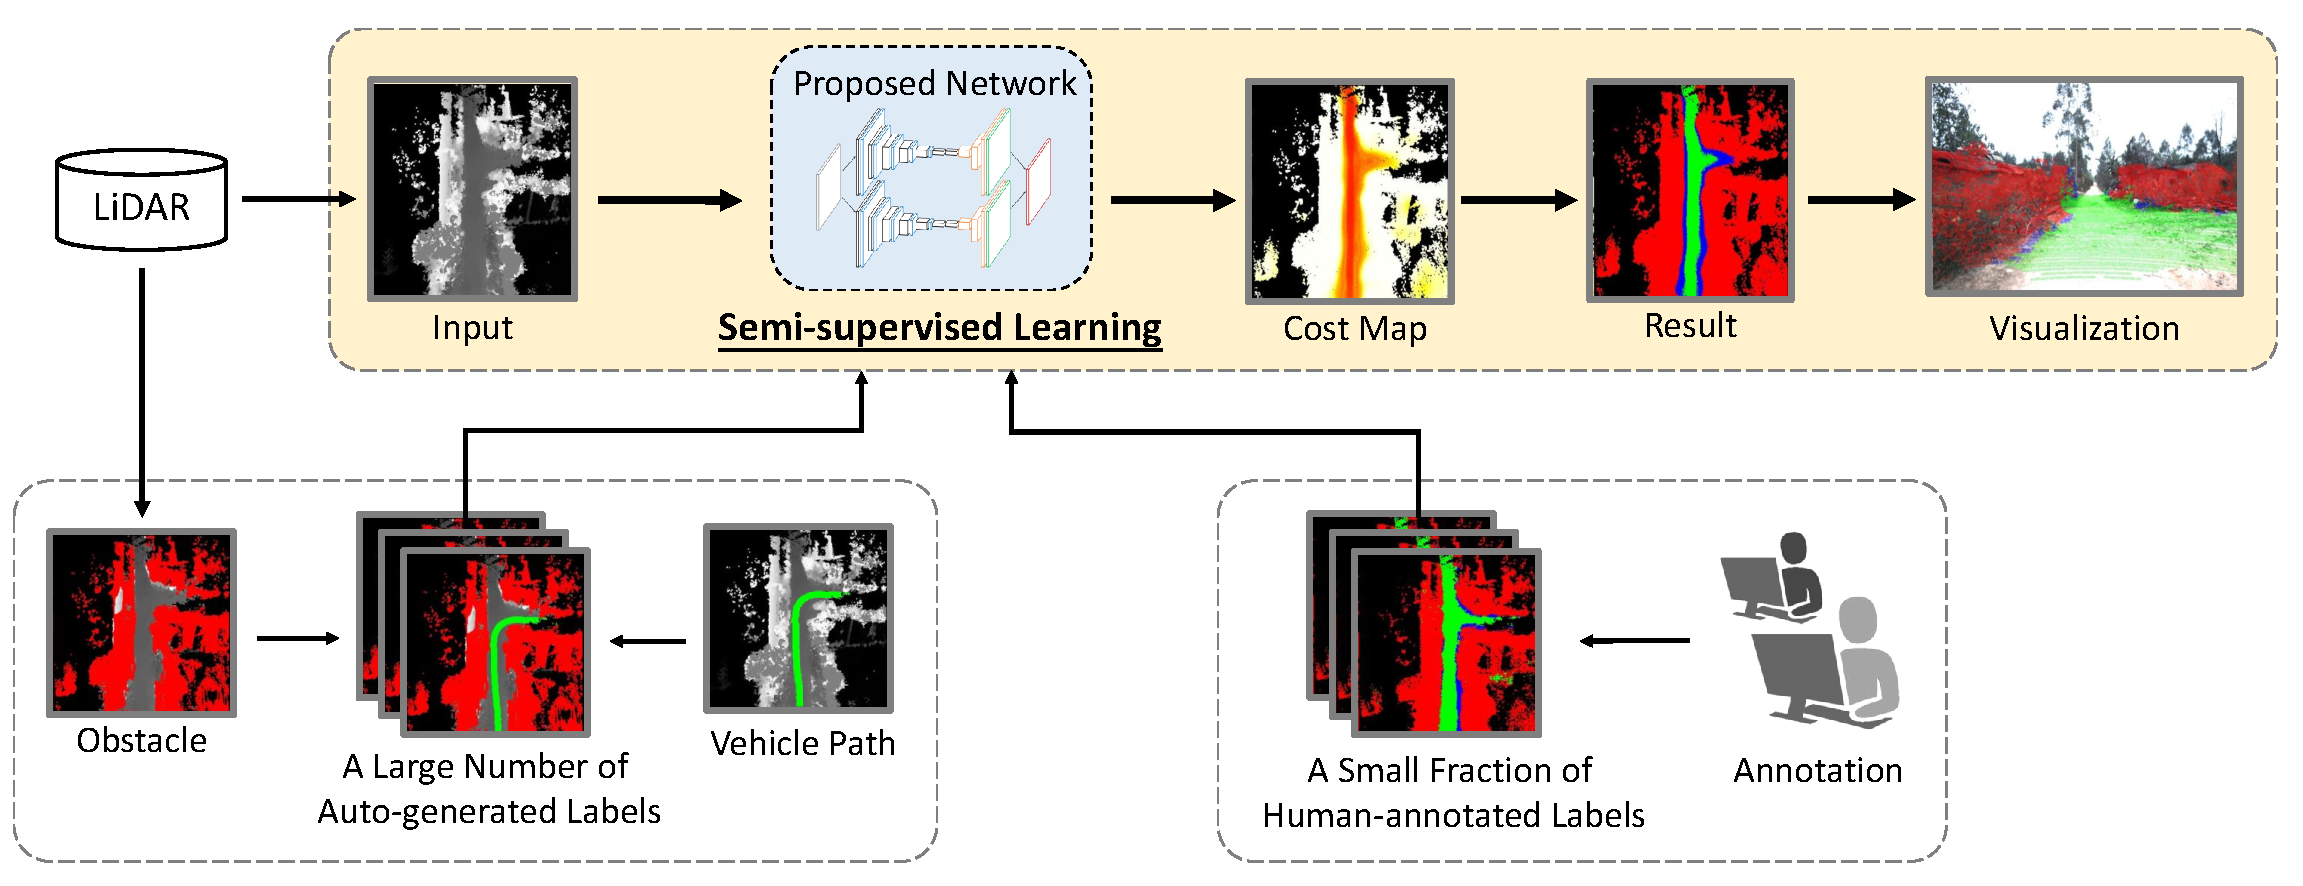
\includegraphics[scale=0.4]{framework.pdf}
	\caption{Overview of the proposed off-road drivable area extraction framework}
	\label{fig:framework}
\end{figure*}

In order to reduce the demand of the high-cost human-annotated data, we propose a semi-supervised learning method shown in Fig.\ref{fig:framework}. This framework can use a large number of auto-generated labels and only a small fraction of human-annotated labels to train the network.

For human-annotated data $X_h$, we use the loss function Equation (\ref{equ:loss0}) for training. For data $X_w$ with only auto-generated weakly labels, we define the loss  $L_{semi}^{br}$ in branch $br$ as below:

\begin{equation}
\label{equ:loss1}
L^{br}_{semi}(X_w;\Theta^{br})=-\lambda \sum_{j}{\widetilde{y_j^{br}} \log{P(y_j^{br}|\Theta^{br})}}
\end{equation}

where $\widetilde{y_j} \in \widetilde{Y}$ denotes the auto-generated labels and $\lambda$ is a regularization weight.

When training the network with human-annotated labels and auto-generated labels simultaneously, combine the Equation (\ref{equ:loss0}) and Equation (\ref{equ:loss1}) together.

\begin{equation}
\label{equ:loss2}
L^{br}(X_h,X_w;\Theta^{br})=L^{br}(X_h;\Theta^{br})+L^{br}_{semi}(X_w;\Theta^{br})
\end{equation}

In each training batch, the mean loss of human-annotated and auto-generated data will be used for back propagation.

\section{IMPLEMENTATION DETAILS}

\subsection{Training Setup}

\subsection{Ground Truth Labeling}

\subsection{Evaluation}

\section{EXPERIMENTAL RESULTS}	\label{sec:experiment}

\subsection{Data set}

\subsection{Proposed Method Results}

\begin{figure*}[ht]
	\centering
	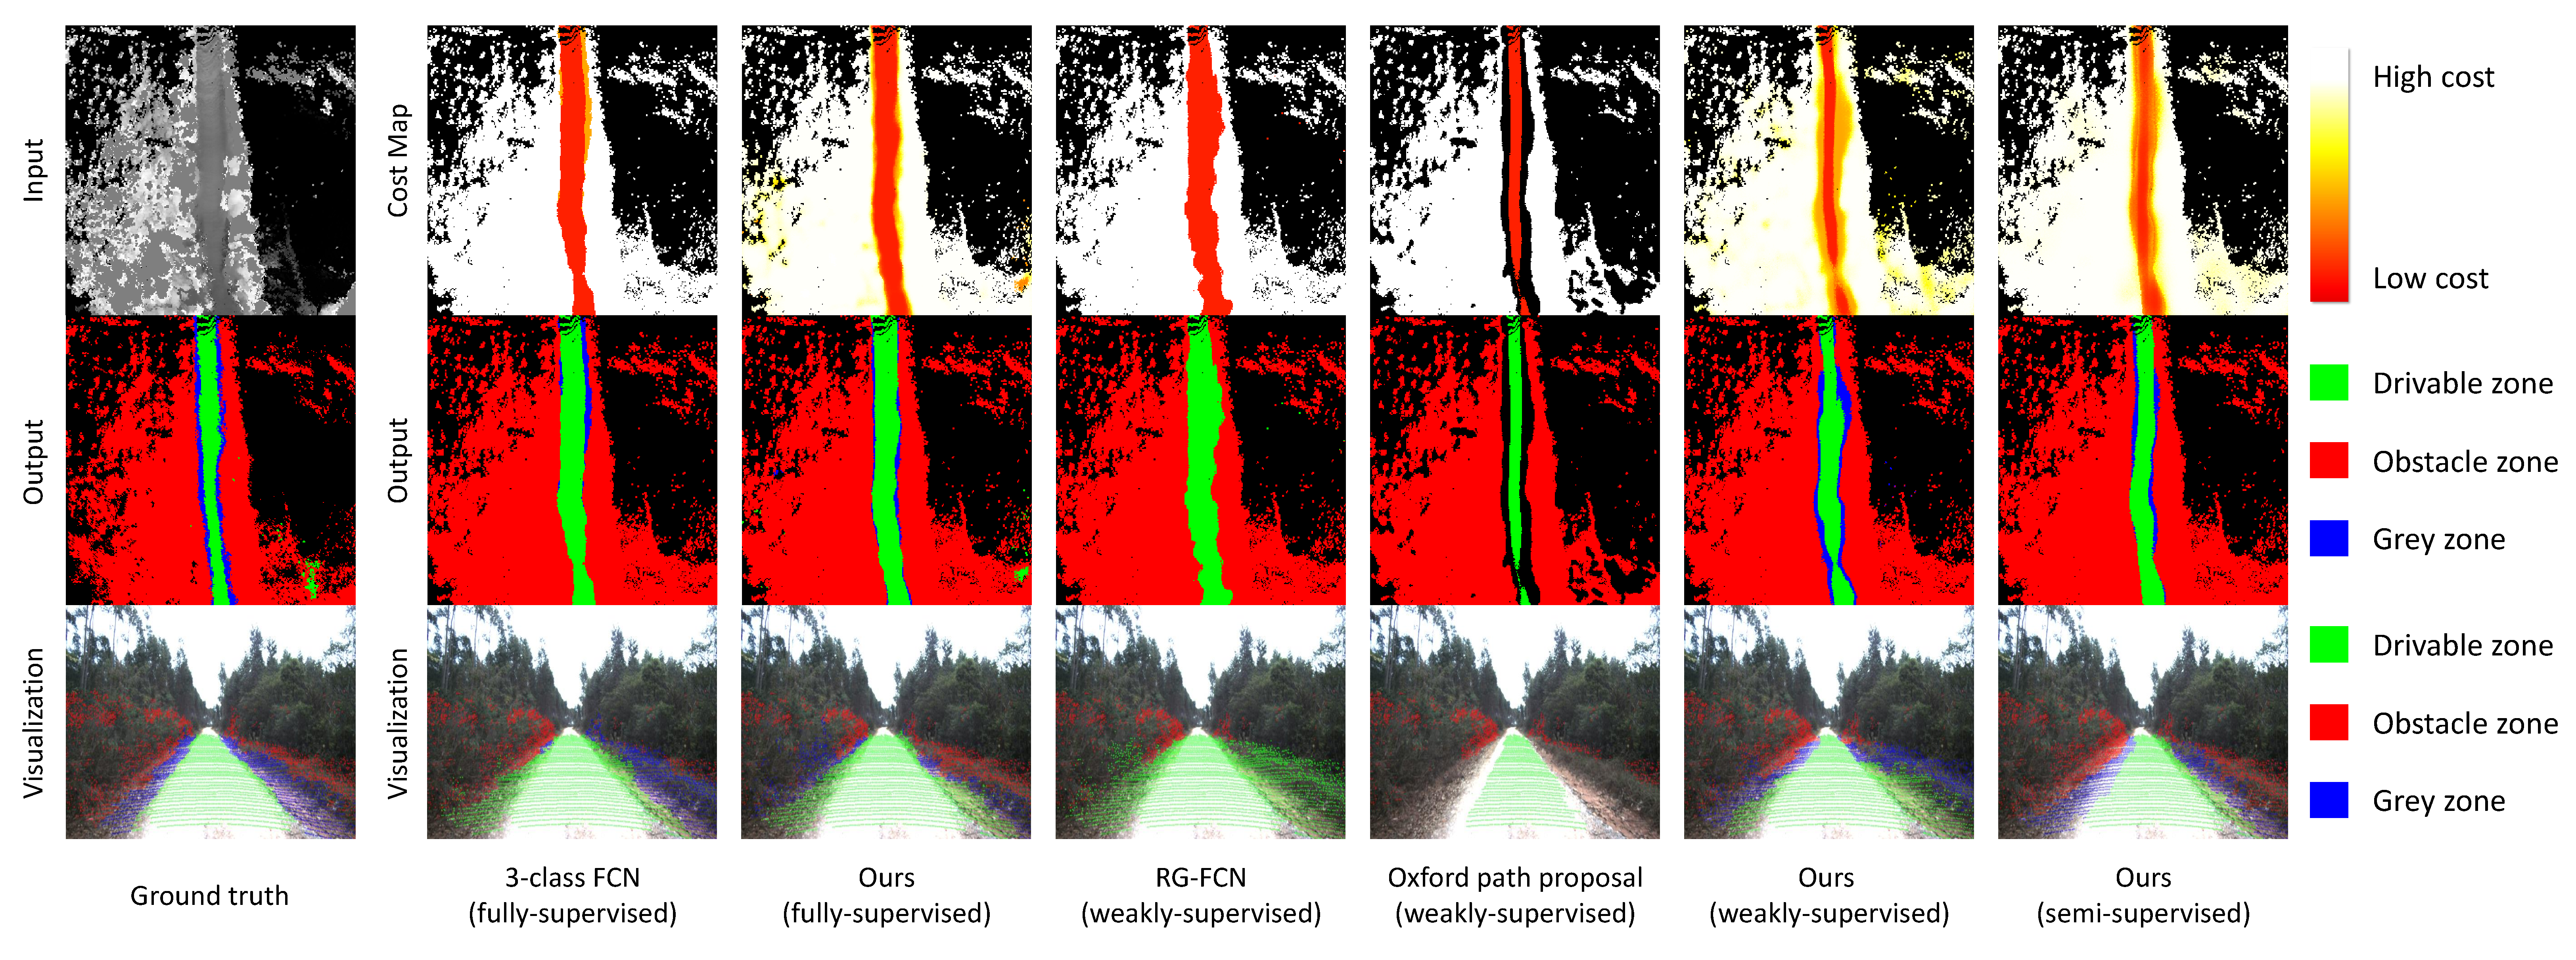
\includegraphics[scale=0.17]{straightRoad.pdf}
	\caption{Qualitative results at straight road scene.}
	\label{fig:straight_road}
\end{figure*}

\begin{figure*}[h]
	\centering
	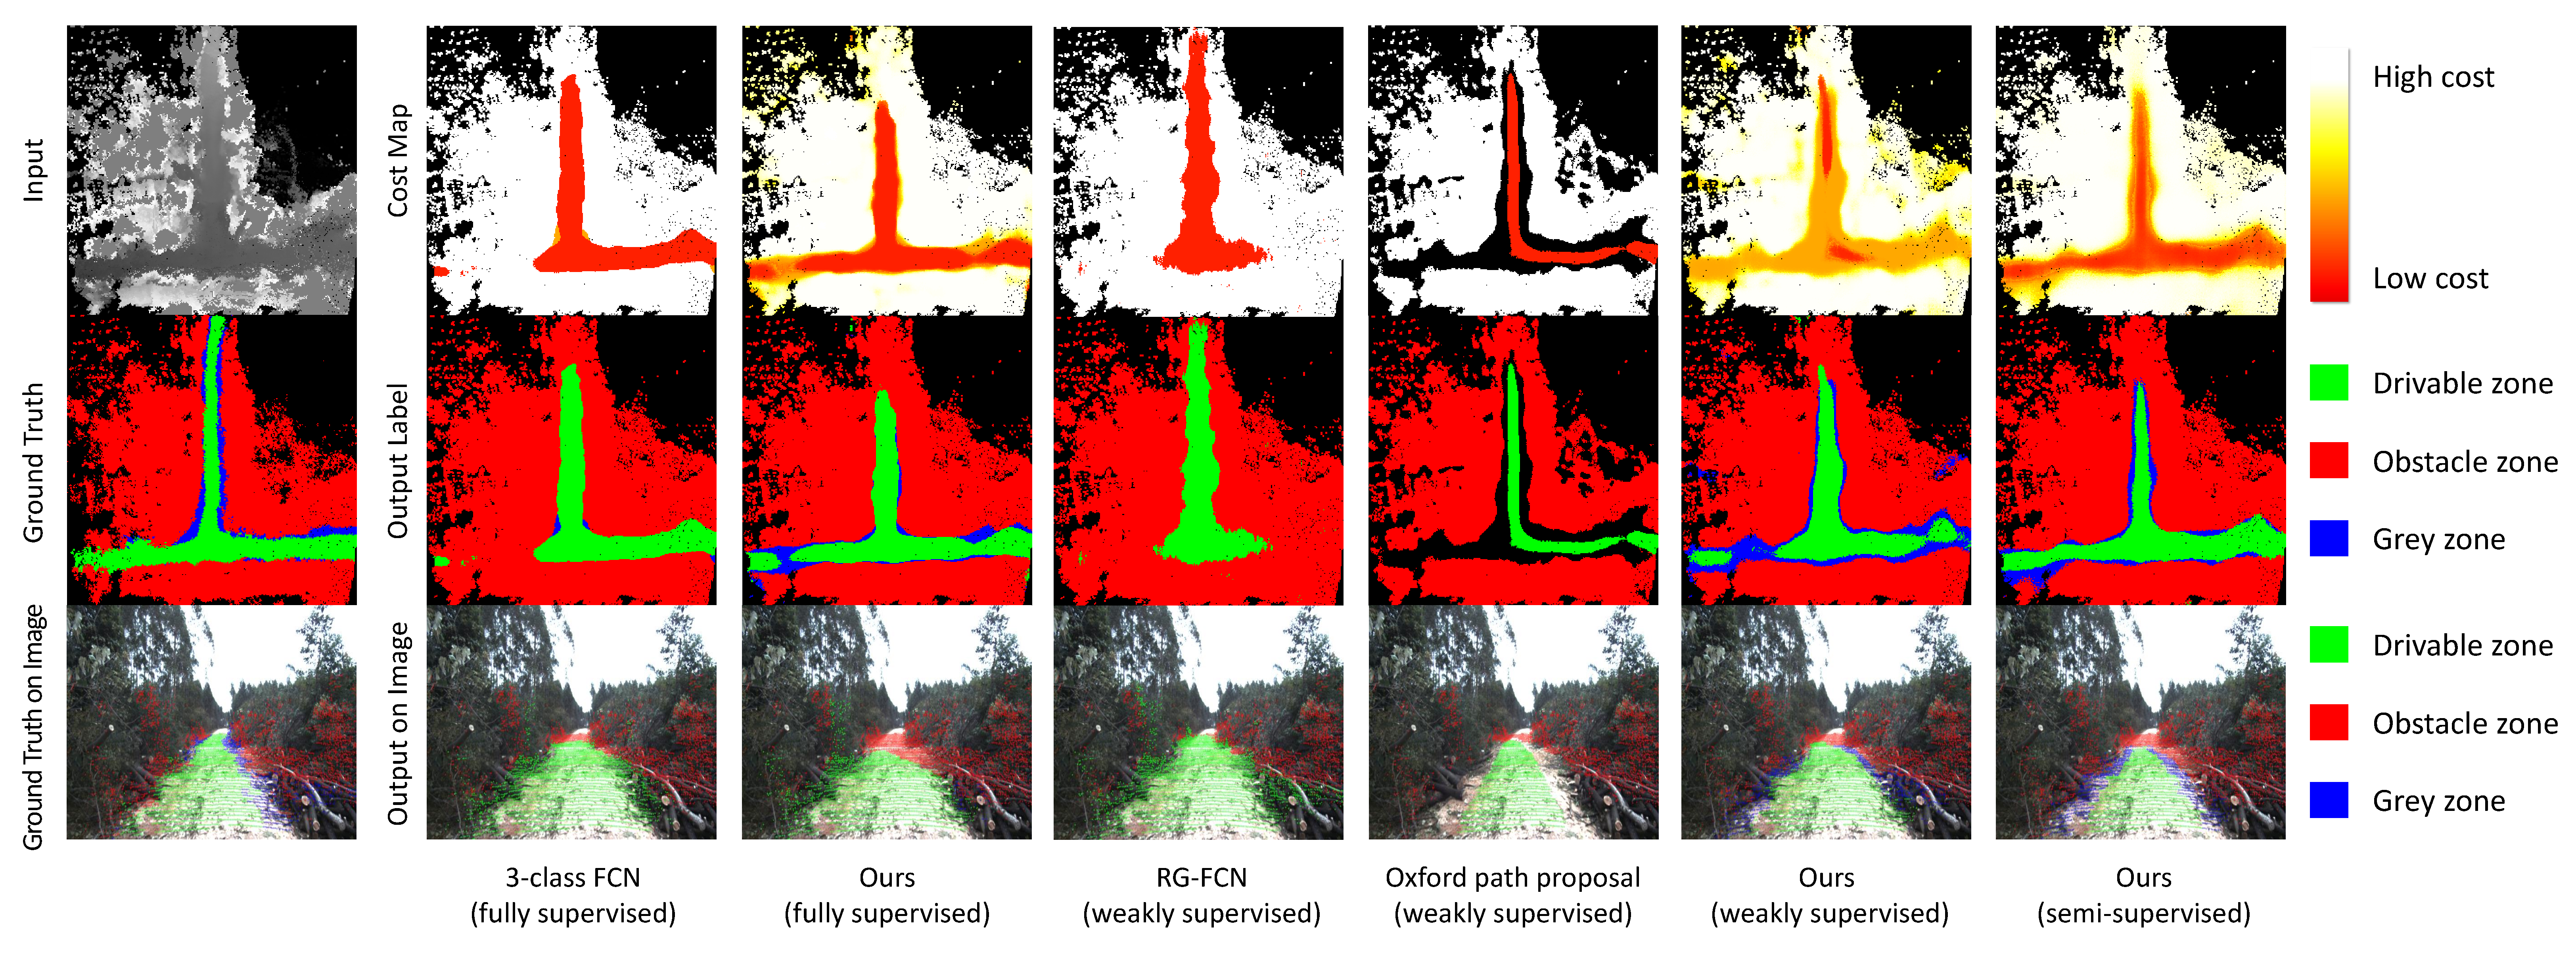
\includegraphics[scale=0.17]{crossRoad.pdf}
	\caption{Qualitative results at cross road scene.}
	\label{fig:cross_road}
\end{figure*}


\begin{figure}[h]
	\centering
	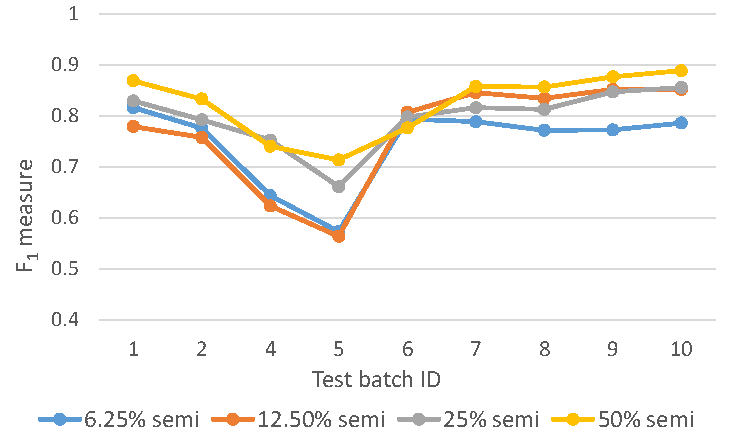
\includegraphics[scale=0.6]{semiSupvisedResult.pdf}
	\caption{Quantitative comparison on test set.}
	\label{fig:semi_curve}
\end{figure}

\begin{table*}
	\caption{Evaluation Measures}
	\label{tab:evaluation}
	\centering
	\renewcommand{\arraystretch}{1.7}
	\begin{tabular}{cclccl}
		\hline
		\multicolumn{3}{c|}{Drivable Zone}                                                                                                    & \multicolumn{3}{c}{Obstacle Zone}                                                                                                  \\ \hline
		Definition                                            & \multicolumn{2}{c|}{Explanation}                                               & Definition                                          & \multicolumn{2}{c}{Explanation}                                               \\ \hline
		$Q_1={TP(G_{dri})}/{\Arrowvert Y_{dri} \Arrowvert}$   & \multicolumn{2}{c|}{$TP(G_{dri})=\Arrowvert G_{dri}\cap Y_{dri} \Arrowvert$}   & $Q_1={TP(G_{obs})}/{\Arrowvert Y_{obs} \Arrowvert}$ & \multicolumn{2}{c}{$TP(G_{obs})=\Arrowvert G_{obs}\cap Y_{obs} \Arrowvert$}   \\
		$Q_2={TP(G_{dri})}/{\Arrowvert G_{dri} \Arrowvert}$   & \multicolumn{2}{c|}{$TP(G_{dri})=\Arrowvert G_{dri}\cap Y_{dri} \Arrowvert$}   & $Q_2={TP(G_{obs})}/{\Arrowvert G_{obs} \Arrowvert}$ & \multicolumn{2}{c}{$TP(G_{obs})=\Arrowvert G_{obs}\cap Y_{obs} \Arrowvert$}   \\
		$Q_3={TP(VP_{dri})}/{\Arrowvert VP_{dri} \Arrowvert}$ & \multicolumn{2}{c|}{$TP(VP_{dri})=\Arrowvert VP_{dri}\cap Y_{dri} \Arrowvert$} & /                                                   & \multicolumn{2}{c}{/}                                                         \\
		$F_1={2Q_1Q_2}/{(Q_1+Q_2)}$                           & \multicolumn{2}{c|}{$F_1 $ Measure}                                            & $F_1={2Q_1Q_2}/{(Q_1+Q_2)}$                         & \multicolumn{2}{c}{$F_1$ Measure}                                             \\ 
		\hline
	\end{tabular}
	\renewcommand{\arraystretch}{2.3}
	\begin{tabular}{llllll}
		\textbf{dri}: Drivable zone                 & \textbf{obs}: Obstacle zone              & \textbf{G}: Ground truth                            & \textbf{Y}: Prediction & \textbf{VP}: Vehicle Path & $\Arrowvert \textbf{X}\Arrowvert$: Pixel number in X \\
	\end{tabular}
\end{table*}

\begin{table*}
	\caption{quantitative evaluation of different methods}
	\label{tab:all_result}
	\centering
	\renewcommand{\arraystretch}{1.7}
	\begin{tabular}{c|cccc|ccc}
		\hline
		& \multicolumn{4}{c|}{Drivable zone}                                & \multicolumn{3}{c}{Obstacle zone}               \\ \cline{2-8} 
		& $Q_1$ (PRE)    & $Q_2$ (REC)    & $Q_3$ (ACC)    & $F_1$          & $Q_1$ (PRE)    & $Q_2$ (REC)    & $F_1$          \\ \hline
		3-class FCN (fully-sup.) & 74.93          & 82.99          & \textbf{98.92} & 78.75          & 94.36          & \textbf{98.44} & 96.36          \\
		Ours (fully-sup.)        & \textbf{76.01} & \textbf{86.72} & 98.09          & \textbf{81.01} & \textbf{96.20} & 96.75          & \textbf{96.47} \\ \hline
		RG-FCN (weakly-sup.)     & 59.78          & {79.15}        & 93.16          & 68.11          & 94.46          & {95.38}        & 94.92          \\
		Oxford PP (weakly-sup.)  & \textbf{97.00} & 47.38          & 83.71          & 63.66          & \textbf{98.40} & 89.84          & 93.93          \\
		Ours (weakly-sup.)       & 72.38          & 78.83          & {95.21}        & {75.47}        & {96.31}        & 94.84          & {95.57}        \\
		Ours (semi-sup.)         & {81.73}        & \textbf{81.73} & \textbf{96.24} & \textbf{81.73} & 95.60          & \textbf{97.38} & \textbf{96.49} \\ \hline
	\end{tabular}
\end{table*}

\begin{table*}
	\caption{quantitative comparison of $F_1$ measure}
	\label{tab:semic}
	\centering
	\renewcommand{\arraystretch}{1.7}
	\begin{tabular}{c|ccccc}
		\hline
		- & 6.25\% semi-sup. & 12.5\% semi-sup. & 25\% semi-sup. & 50\% semi-sup. & Fully-sup.	\\
		\hline
		$F_1$ measure & 73.86 & 75.04 & 78.96 & \textbf{81.73} & 81.01 	\\
		\hline
	\end{tabular}
\end{table*}

\subsection{Limitations}

\section{CONCLUSION}

nothing

\addtolength{\textheight}{-12cm}   % This command serves to balance the column lengths
                                  % on the last page of the document manually. It shortens
                                  % the textheight of the last page by a suitable amount.
                                  % This command does not take effect until the next page
                                  % so it should come on the page before the last. Make
                                  % sure that you do not shorten the textheight too much.

%%%%%%%%%%%%%%%%%%%%%%%%%%%%%%%%%%%%%%%%%%%%%%%%%%%%%%%%%%%%%%%%%%%%%%%%%%%%%%%%



%%%%%%%%%%%%%%%%%%%%%%%%%%%%%%%%%%%%%%%%%%%%%%%%%%%%%%%%%%%%%%%%%%%%%%%%%%%%%%%%



%%%%%%%%%%%%%%%%%%%%%%%%%%%%%%%%%%%%%%%%%%%%%%%%%%%%%%%%%%%%%%%%%%%%%%%%%%%%%%%%
\section*{APPENDIX}


\section*{ACKNOWLEDGMENT}

nothing.

\begin{thebibliography}{99}

\bibitem{c1} G. O. Young, �Synthetic structure of industrial plastics (Book style with paper title and editor),� 	in Plastics, 2nd ed. vol. 3, J. Peters, Ed.  New York: McGraw-Hill, 1964, pp. 15�64.

\end{thebibliography}




\end{document}
